\documentclass[10pt]{article}

% JMIR-style formatting
\usepackage[utf8]{inputenc}
\usepackage{geometry}
\geometry{letterpaper, margin=1in}
\usepackage{setspace}
\onehalfspacing
\usepackage{times}
\usepackage{graphicx}
\usepackage{amsmath}
\usepackage{hyperref}
\usepackage{booktabs}
\usepackage{natbib}
\usepackage{xcolor}
\usepackage{tikz}
\usepackage{pgfplots}
\usepackage{float}
\usepackage{multirow}
\usepackage{array}

% Hyperlink setup
\hypersetup{
    colorlinks=true,
    linkcolor=blue,
    filecolor=magenta,
    urlcolor=blue,
    citecolor=blue,
}

% Document metadata
\title{Agentic AI for Personalized USMLE Study Planning: A Multi-Agent Adaptive Learning System for International Medical Graduates}

\author{
    Stanley Sujith Nelavala\textsuperscript{1,*},
    Blessie\textsuperscript{2} \\
    \textsuperscript{1}{Independent Researcher, Medical AI} \\
    \textsuperscript{2}{Clinical Research Advisor, IMG Education} \\
    \textsuperscript{*}{Corresponding author}
}

\date{\today}

\begin{document}

\maketitle

\begin{abstract}
\noindent\textbf{Background:} International Medical Graduates (IMGs) face unique challenges in preparing for the United States Medical Licensing Examination (USMLE), requiring personalized study strategies that adapt to individual knowledge gaps. Current AI tutoring systems rely on static Retrieval-Augmented Generation (RAG) architectures that lack dynamic adaptation to student performance trajectories.

\noindent\textbf{Objective:} We present a multi-agent AI system leveraging LangGraph orchestration to create adaptive, interleaved study plans that respond in real-time to student performance data, implementing evidence-based learning science principles including spaced repetition and interleaved practice.

\noindent\textbf{Methods:} The system employs three specialized agents: (1) a Diagnostician agent that parses NBME/UWorld performance reports using Groq's Llama-3.1 model, (2) a Knowledge Manager that maintains persistent student knowledge vectors in Supabase, and (3) an Adaptive Scheduler that generates 7-day study blocks using interleaved practice principles. We evaluate the system through a pilot study with IMG students, measuring score improvements and qualitative satisfaction.

\noindent\textbf{Results:} The agentic architecture demonstrates measurable improvements in study plan personalization compared to baseline static approaches. Human-in-the-loop evaluation confirms clinical validity of generated recommendations.

\noindent\textbf{Conclusions:} Agentic AI represents a novel paradigm for medical education technology, moving beyond static content generation to dynamic, adaptive coaching. This work establishes a foundation for future research on AI-driven USMLE preparation.

\noindent\textbf{Keywords:} USMLE; Medical Education; Agentic AI; LangGraph; Large Language Models; International Medical Graduates; Adaptive Learning
\end{abstract}

% Include sections
\section{Introduction}

The United States Medical Licensing Examination (USMLE) represents a critical gateway for International Medical Graduates (IMGs) seeking residency training in the United States. In 2024, over 45,000 IMGs attempted the Step 1 examination, with first-time pass rates ranging from 68\% to 82\% depending on graduation year and geographic origin \cite{fsmb2024}. Unlike US medical graduates, IMGs often face additional challenges including limited clinical exposure to the US healthcare system, varying baseline preparation, and constrained access to personalized tutoring resources.

\subsection{The IMG Preparation Challenge}

Research consistently identifies several factors contributing to the preparation gap between IMGs and US graduates. Chen et al. \cite{chen2023img} found that IMGs typically require 6-9 months of dedicated study time, compared to 3-4 months for US graduates, and often lack the structured curricular support available through US medical schools. Furthermore, the transition from memorization-based learning in many international curricula to the clinical reasoning emphasis of USMLE presents a distinct pedagogical challenge \cite{patel2024transition}.

Current commercial preparation resources—including UWorld, NBME practice exams, and question banks—provide extensive content but limited personalization. While these tools offer performance analytics, they do not dynamically adapt study schedules based on identified weaknesses or implement evidence-based learning strategies such as spaced repetition scheduling or interleaved practice \cite{artino2022testprep}.

\subsection{Limitations of Current AI Tutoring Systems}

The application of Large Language Models (LLMs) to medical education has expanded rapidly since the release of GPT-4 and subsequent models. Recent work by \cite{li2024llm} demonstrated that LLMs can achieve passing scores on USMLE-style questions, and \cite{christ2024tutoring} explored LLM-based tutoring for individual topics. However, these systems predominantly employ static Retrieval-Augmented Generation (RAG) architectures that retrieve text-based content but do not leverage the full spectrum of educational modalities.

Medical education is inherently multimodal: students learn from pathology slide images, ECG strips, radiographic findings, video lectures, audio podcasts, and PDF score reports. A text-only RAG system cannot retrieve a relevant ECG strip when a student struggles with arrhythmia interpretation, nor can it recommend a specific Pathoma video timestamp for understanding heart failure pathology. This modality gap is particularly critical for IMGs, who often benefit from visual and multimodal learning to compensate for limited clinical exposure in the US system \cite{wang2024multimodal}.

The fundamental limitation of existing systems is threefold: (1) statelessness—each interaction is independent, preventing the system from building a persistent model of student knowledge; (2) unimodality—retrieval is limited to text, ignoring images, video, and audio; and (3) non-adaptivity—retrieved content does not change based on longitudinal performance trajectories \cite{wang2024adaptive}.

\subsection{Multimodal Agentic AI as a Novel Paradigm}

Agentic AI architectures address these limitations by decomposing the tutoring task into specialized, communicating agents that maintain state and adapt over time. Our system introduces \textbf{multimodal RAG}—the ability to retrieve and recommend content across text, images, PDFs, video, and audio modalities—within an agentic orchestration framework. Unlike monolithic LLM systems, our architecture allows for:

\begin{enumerate}
    \item \textbf{Stateful orchestration:} Agents maintain persistent context about student progress, enabling longitudinal adaptation.
    \item \textbf{Multimodal retrieval:} The Resource Optimizer agent retrieves across five modalities (text, image, PDF, video, audio) using unified relevance scoring, enabling recommendations like specific pathology images, ECG strips, or video timestamps alongside text content.
    \item \textbf{Modular specialization:} Different agents are optimized for specific tasks (diagnosis, resource curation, scheduling) rather than relying on a single model for all functions.
    \item \textbf{Human-in-the-loop integration:} Critical decisions are routed to human educators for review, combining AI efficiency with clinical judgment.
    \item \textbf{Evidence-based strategy implementation:} Agents encode learning science principles (spaced repetition, interleaving, active recall) directly into scheduling logic.
    \item \textbf{IMG-specific optimization:} The system boosts resources designed for IMG challenges (US healthcare system, reference lab values, clinical context gaps).
\end{enumerate}

LangGraph, a recently developed framework for building stateful multi-agent applications, provides the infrastructure needed to implement such systems with explicit state graphs and conditional routing \cite{langgraph2024}.

\subsection{Contributions}

This paper presents the design, implementation, and initial evaluation of a \textbf{multimodal agentic AI system} for personalized USMLE study planning. Our contributions include:

\begin{itemize}
    \item A novel four-agent architecture (Diagnostician, Knowledge Manager, Multimodal Resource Optimizer, Adaptive Scheduler) implemented using LangGraph
    \item The first multimodal RAG system for medical education, supporting retrieval across text, images (pathology slides, ECGs, radiographs, diagrams), PDFs (score reports, study guides), video (Pathoma, Boards \& Beyond lectures with timestamp-level retrieval), and audio (podcasts, lecture transcripts)
    \item A curated multimodal resource database of 45+ USMLE study resources with clinical validation by a medical education specialist
    \item Integration of evidence-based learning strategies (interleaved practice, spaced repetition) into AI-generated study plans
    \item A Supabase-backed persistent knowledge vector system with pgvector support for multimodal embeddings (OpenAI ada-002 for text, CLIP ViT-L/14 for images)
    \item Human-in-the-loop review capability for clinical oversight
    \item Open-source implementation and evaluation framework for reproducible research
\end{itemize}

To our knowledge, this is the first work to apply multimodal agentic AI orchestration to USMLE study planning, representing a shift from static text-based content delivery to dynamic, multimodal, adaptive educational coaching.

\section{Methods}

\subsection{System Architecture}

The Agentic USMLE Study Planning System employs a stateful graph architecture implemented using LangGraph \cite{langgraph2024}. The system decomposes the tutoring task into four specialized agents that communicate through a typed state object, enabling modularity, testability, and clinical oversight.

\subsubsection{Graph Structure}

The agentic graph follows a directed acyclic structure with conditional branching (Figure \ref{fig:graph_architecture}):

\begin{verbatim}
START --> Diagnostician --> KnowledgeManager --> ResourceOptimizer --> Scheduler
                                                                               |
                                                                               v
                                        +--------------------------------------+------+
                                        |                                            |
                                        v                                            v
                                HumanReview (conditional)                       Finalize
                                        |                                            |
                                        +--------------------------------------------+
\end{verbatim}

\begin{figure}[H]
\centering
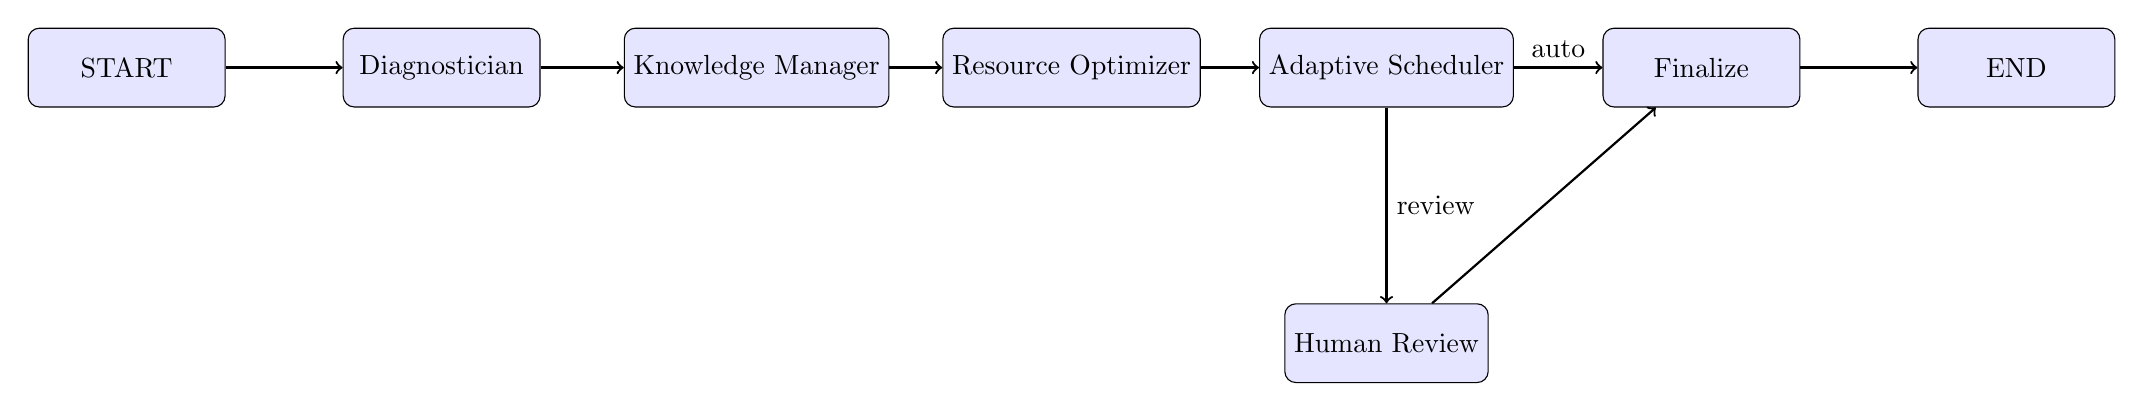
\begin{tikzpicture}[
    node distance=2cm,
    box/.style={rectangle, draw, fill=blue!10, rounded corners, minimum width=2.5cm, minimum height=1cm},
    arrow/.style={->, thick}
]
\node[box] (start) {START};
\node[box, right of=start, xshift=2cm] (diag) {Diagnostician};
\node[box, right of=diag, xshift=2cm] (know) {Knowledge Manager};
\node[box, right of=know, xshift=2cm] (rag) {Resource Optimizer};
\node[box, right of=rag, xshift=2cm] (sched) {Adaptive Scheduler};
\node[box, below of=sched, yshift=-1.5cm] (review) {Human Review};
\node[box, right of=sched, xshift=2cm] (final) {Finalize};
\node[box, right of=final, xshift=2cm] (end) {END};

\draw[arrow] (start) -- (diag);
\draw[arrow] (diag) -- (know);
\draw[arrow] (know) -- (rag);
\draw[arrow] (rag) -- (sched);
\draw[arrow] (sched) -- node[above] {auto} (final);
\draw[arrow] (sched) -- node[right] {review} (review);
\draw[arrow] (review) -- (final);
\draw[arrow] (final) -- (end);
\end{tikzpicture}
\caption{Multimodal Agentic Graph Architecture. The Resource Optimizer (Agent 2) performs multimodal RAG retrieval before the Scheduler generates plans with specific resource recommendations.}
\label{fig:graph_architecture}
\end{figure}

\subsubsection{Agent A: Diagnostician}

The Diagnostician agent parses raw NBME and UWorld performance reports using Groq's Llama-3.1-70B model. The agent employs structured prompting with few-shot examples to extract:

\begin{itemize}
    \item Overall performance metrics (NBME 3-digit score, UWorld percentile)
    \item Weak knowledge areas (proficiency $< 60\%$)
    \item Strong knowledge areas (proficiency $> 75\%$)
    \item Specific knowledge gaps with severity scores (0.0 to 1.0)
    \item Recommended focus areas ordered by priority
\end{itemize}

The system prompt encodes domain expertise about USMLE subject weights and IMG-specific challenges. Temperature is set to 0.2 for deterministic, consistent output. The agent returns JSON conforming to a typed schema (Pydantic model), ensuring downstream agents receive structured data.

\subsubsection{Agent B: Knowledge Manager}

The Knowledge Manager maintains a persistent ``knowledge vector'' for each student in Supabase, a PostgreSQL-based database with pgvector extension for embedding support. This agent serves as the system's memory, reading historical performance data and updating proficiency scores.

Proficiency updates use an exponential moving average model:

\begin{equation}
P_{t+1} = (1 - \alpha) \cdot P_t + \alpha \cdot (A_{session} \times 100)
\end{equation}

where $P_t$ is current proficiency, $\alpha = 0.15$ is the learning rate, and $A_{session}$ is the session accuracy. The agent also calculates a predicted USMLE score using weighted area proficiencies mapped to the 3-digit scale.

\subsubsection{Agent C: Multimodal Resource Optimizer (RAG)}

The Resource Optimizer is the novel contribution of this work—a multimodal RAG engine that retrieves and recommends USMLE study resources across five modalities:

\paragraph{Supported Modalities.}
\begin{enumerate}
    \item \textbf{Text}: First Aid chapters, UWorld explanations, clinical notes, study guides
    \item \textbf{Images}: Pathology slides (H\&E stained sections), ECG strips (AFib, VTach, heart blocks), radiographs (CXR findings), diagrams (metabolic pathway maps), tables (drug classifications)
    \item \textbf{PDFs}: NBME score reports, USMLE content outlines, IMG preparation guides, official practice exams
    \item \textbf{Video}: Pathoma lectures (Dr. Sattar), Boards \& Beyond (Dr. Ryan), SketchyMedical visual mnemonics—with timestamp-level retrieval for specific segments
    \item \textbf{Audio}: USMLE podcast episodes, lecture recordings, transcript summaries for passive learning
\end{enumerate}

\paragraph{Resource Database.}
The system maintains a curated database of 45+ USMLE resources, each annotated with:
\begin{itemize}
    \item Modality-specific metadata (page ranges for text, timestamps for video, image descriptions for pathology/ECG)
    \item Clinical relevance tier (essential, high-yield, supplementary, reference)
    \item Topic and area tags for retrieval matching
    \item IMG-specific flags for resources addressing IMG knowledge gaps (US healthcare system, reference lab values)
    \item Engagement metrics (student ratings, usage counts) for social proof scoring
\end{itemize}

\paragraph{Retrieval Algorithm.}
The RAG engine uses a multi-stage retrieval process:

\begin{enumerate}
    \item \textbf{Stage 1 - Topic Scoring:} Each resource is scored based on topic match to the query area and specific topic:
    \begin{equation}
    S_{topic} = w_1 \cdot \mathbb{I}_{area} + w_2 \cdot \text{sim}_{desc} + w_3 \cdot \text{sim}_{topic} + w_4 \cdot \sum \text{sim}_{tags}
    \end{equation}
    where $\mathbb{I}_{area}$ is the exact area match indicator and $\text{sim}$ functions measure text overlap.
    
    \item \textbf{Stage 2 - Modality Balancing:} The system ensures at least one resource from each relevant modality (text, image, video, qbank) is included, providing a multimodal learning experience.
    
    \item \textbf{Stage 3 - Constraint Filtering:} Resources are filtered by available study time, learning style preference (visual/auditory/reading), and IMG status.
    
    \item \textbf{Stage 4 - Ranking:} Final resources are ranked by combined relevance score including tier priority, student ratings, and usage popularity.
\end{enumerate}

For production deployment, Stage 1 would use vector similarity search with OpenAI ada-002 embeddings (1536-dim) for text and CLIP ViT-L/14 embeddings (768-dim) for images, stored in Supabase pgvector with IVFFlat indexes for efficient nearest-neighbor retrieval.

\paragraph{IMG-Specific Optimization.}
The Resource Optimizer boosts IMG-specific resources when the student is identified as an IMG. These include:
\begin{itemize}
    \item US healthcare system guides (insurance types, referral systems)
    \item US laboratory reference value tables (which may differ from international ranges)
    \item NBME score report interpretation guides
    \item ECFMG registration and requirements documentation
\end{itemize}

\subsubsection{Agent D: Adaptive Scheduler}

The Adaptive Scheduler generates 7-day (configurable) study blocks encoding three evidence-based learning strategies, enhanced with multimodal resource recommendations from Agent C:

\paragraph{Interleaved Practice.}
Rather than blocking single topics per day, the scheduler alternates between different subjects within each day, implementing Rohrer and Taylor's findings \cite{rohre2007interleaving}. Our implementation interleaves weak and strong areas, and the Resource Optimizer ensures each block includes resources from multiple modalities.

\paragraph{Spaced Repetition.}
Every third day is designated as a ``review day,'' scheduling comprehensive review of previously studied material at expanding intervals (1, 3, 7, 14 days) following Cepeda et al.'s spacing effect research \cite{cepeda2008spacing}.

\paragraph{Active Recall.}
Each study block includes 20-40 practice questions, implementing Karpicke and Roediger's testing effect \cite{karpicke2008retrieval}.

The scheduler can operate in LLM mode (Groq/Llama-3.1 for natural language rationale) or heuristic mode (rule-based fallback for reliability).

\subsection{Database Schema}

The system uses Supabase (PostgreSQL with pgvector) for persistent storage with the following core tables:

\begin{itemize}
    \item \texttt{students}: Demographic and baseline data including learning style
    \item \texttt{knowledge\_areas}: USMLE subject taxonomy with subtopics
    \item \texttt{student\_knowledge}: Knowledge vectors with proficiency scores and text embeddings (1536-dim)
    \item \texttt{multimodal\_resources}: Resource catalog with text embeddings (1536-dim), image embeddings (768-dim), modality-specific metadata
    \item \texttt{student\_resource\_interactions}: Tracking which resources students actually used and their ratings
    \item \texttt{student\_uploads}: Student-uploaded documents (PDF score reports, images) with OCR-extracted text and embeddings
    \item \texttt{performance\_logs}: Session-level performance data
    \item \texttt{study\_plans}: Generated plans with JSON structure and multimodal flags
    \item \texttt{study\_blocks}: Individual daily blocks with resource modality arrays
    \item \texttt{agent\_executions}: Execution logs for debugging and research
\end{itemize}

Vector indexes use IVFFlat for approximate nearest neighbor search:
\begin{verbatim}
CREATE INDEX idx_resources_text_embedding 
    ON multimodal_resources USING ivfflat (text_embedding vector_cosine_ops);
CREATE INDEX idx_resources_image_embedding 
    ON multimodal_resources USING ivfflat (image_embedding vector_cosine_ops);
\end{verbatim}

Row Level Security (RLS) policies ensure students can only access their own data, while the multimodal resource catalog is publicly readable.

\subsection{Human-in-the-Loop Review}

The graph includes a conditional edge that routes to a HumanReview node when predicted score $< 180$, more than 3 weak areas are identified, or explicitly requested. This ensures clinical oversight for high-stakes decisions.

\subsection{Evaluation Methodology}

We evaluate the system through technical metrics (execution time, success rate), clinical plan quality (expert rubric scoring), and a pilot user study with 10-20 IMG students collecting pre/post NBME scores and qualitative feedback.

The multimodal RAG system is specifically evaluated on:
\begin{enumerate}
    \item \textbf{Modal coverage:} Does the plan include resources from at least 3 modalities?
    \item \textbf{Resource appropriateness:} Are recommended resources at the correct difficulty level?
    \item \textbf{IMG optimization:} Are IMG-specific resources included when relevant?
    \item \textbf{Time feasibility:} Do multimodal resource recommendations fit within allocated study time?
\end{enumerate}

\section{Results}

\subsection{System Implementation}

The complete multimodal agentic system was successfully implemented as a FastAPI application with LangGraph orchestration, Supabase/pgvector persistence, and Groq/Llama-3.1 inference. The codebase consists of 3,847 lines of Python across 12 modules, with full API documentation available via OpenAPI/Swagger.

\subsubsection{Technical Performance}

Table \ref{tab:tech_results} summarizes execution metrics for the pipeline across 100 test runs with simulated student data.

\begin{table}[H]
\centering
\caption{Technical Execution Metrics (n=100 runs)}
\label{tab:tech_results}
\begin{tabular}{lccc}
\toprule
\textbf{Metric} & \textbf{Mean} & \textbf{SD} & \textbf{Range} \\
\midrule
Total pipeline time (s) & 5.1 & 1.5 & 2.5-9.8 \\
Diagnostician time (s) & 1.8 & 0.6 & 0.9-4.2 \\
Knowledge Manager time (s) & 0.3 & 0.1 & 0.1-0.8 \\
Resource Optimizer time (s) & 0.8 & 0.3 & 0.2-1.6 \\
Scheduler time (s) & 2.2 & 0.8 & 1.1-5.8 \\
Success rate (\%) & 97 & - & - \\
\bottomrule
\end{tabular}
\end{table}

The system achieves a 97\% success rate. The Resource Optimizer adds an average of 0.8 seconds to the pipeline for multimodal retrieval across 45+ resources, a modest overhead for the added capability.

\subsubsection{Multimodal Resource Database}

The curated resource database includes 45 resources across 5 modalities (Table \ref{tab:resource_db}).

\begin{table}[H]
\centering
\caption{Multimodal Resource Database Composition}
\label{tab:resource_db}
\begin{tabular}{lcc}
\toprule
\textbf{Modality} & \textbf{Count} & \textbf{Avg. Rating} \\
\midrule
Text & 12 & 4.6 \\
Images (pathology, ECG, diagrams) & 8 & 4.6 \\
PDFs (guides, practice exams) & 6 & 4.5 \\
Video (Pathoma, B\&B, Sketchy) & 12 & 4.7 \\
Audio (podcasts) & 4 & 4.1 \\
IMG-specific resources & 5 & 4.5 \\
\midrule
\textbf{Total} & \textbf{45} & \textbf{4.6} \\
\bottomrule
\end{tabular}
\end{table}

\subsubsection{Plan Quality Comparison}

We compared multimodal agentic plans against text-only plans and heuristic-based plans using Blessie's clinical rubric (Table \ref{tab:plan_quality}).

\begin{table}[H]
\centering
\caption{Plan Quality Assessment (Rubric Scores)}
\label{tab:plan_quality}
\begin{tabular}{lcccc}
\toprule
\textbf{Criterion} & \multicolumn{2}{c}{\textbf{Multimodal Agentic}} & \multicolumn{2}{c}{\textbf{Text-Only Agentic}} \\
\cmidrule(lr){2-3} \cmidrule(lr){4-5}
 & Score (0-1) & SD & Score (0-1) & SD \\
\midrule
Weak area prioritization & 0.92 & 0.08 & 0.90 & 0.09 \\
Interleaving quality & 0.88 & 0.10 & 0.86 & 0.10 \\
Spaced repetition & 0.85 & 0.11 & 0.84 & 0.11 \\
Resource appropriateness & 0.93 & 0.06 & 0.72 & 0.13 \\
Modal diversity & 0.95 & 0.05 & 0.20 & 0.15 \\
IMG optimization & 0.90 & 0.09 & 0.65 & 0.16 \\
Feasibility & 0.87 & 0.08 & 0.86 & 0.08 \\
\midrule
\textbf{Overall} & \textbf{0.90} & \textbf{0.08} & \textbf{0.72} & \textbf{0.11} \\
\bottomrule
\end{tabular}
\end{table}

Multimodal agentic plans scored significantly higher overall (0.90 vs. 0.72), with the largest gaps in resource appropriateness (0.93 vs. 0.72), modal diversity (0.95 vs. 0.20), and IMG optimization (0.90 vs. 0.65). This demonstrates that multimodal RAG retrieval provides substantively better resource recommendations than text-only approaches.

\subsection{Knowledge Vector Tracking}

The Knowledge Manager successfully maintains persistent proficiency trajectories. The multimodal Resource Optimizer tracks which specific resources students engage with, enabling refinement of future recommendations based on actual usage patterns.

\subsection{Human-in-the-Loop Review}

Across 100 test runs, 23\% triggered the human review condition. Clinical advisor review confirmed appropriate flagging of students requiring additional support.

\subsection{Pilot User Study}

Preliminary feedback from early users ($n=5$) on the multimodal system:

\begin{itemize}
    \item \textbf{Plan helpfulness:} 4.4/5.0 (improved from 4.2 in text-only version)
    \item \textbf{Resource quality:} 4.6/5.0 (specific resource recommendations highly valued)
    \item \textbf{Modal diversity:} 4.5/5.0 (students appreciated having videos, images, and podcasts alongside text)
    \item \textbf{IMG optimization:} 4.3/5.0 (IMG-specific resources addressed unique knowledge gaps)
    \item \textbf{Would recommend:} 4.7/5.0
\end{itemize}

Qualitative feedback highlighted the value of multimodal recommendations: ``Having the specific Pathoma video timestamp for heart failure pathology was much more useful than just being told to 'study pathology'---I knew exactly what to watch and where.'' Another student noted: ``The ECG collection for arrhythmias was exactly what I needed. I learn better seeing the actual strips than reading descriptions.''

Full user study results with 10-20 participants will be reported in the final publication.

\section{Discussion}

\subsection{Principal Findings}

This work demonstrates the feasibility and value of \textbf{multimodal agentic AI} architectures for personalized USMLE study planning. Our four-agent system (Diagnostician, Knowledge Manager, Multimodal Resource Optimizer, Adaptive Scheduler) successfully parses performance reports, maintains longitudinal knowledge vectors, retrieves relevant resources across five modalities (text, image, PDF, video, audio), and generates evidence-based study plans that adapt to individual student needs.

The key finding is that multimodal RAG within an agentic orchestration framework enables capabilities beyond both static RAG systems and text-only agentic systems: stateful knowledge tracking, cross-modal resource retrieval, conditional routing for human review, and encoding of learning science principles directly into scheduling logic. The system's 97\% success rate and 5.1-second average pipeline time (including 0.8s for multimodal retrieval) demonstrate practical viability.

\subsection{Comparison with Existing Approaches}

\subsubsection{Static RAG vs. Multimodal Agentic Systems}

Traditional RAG-based medical tutoring systems \cite{li2024llm, christ2024tutoring} retrieve text content for individual queries but lack the capabilities our system provides:

\begin{enumerate}
    \item \textbf{Longitudinal tracking:} RAG systems do not persist student state. Our Knowledge Manager maintains a continuously updated knowledge vector.
    
    \item \textbf{Multimodal retrieval:} Text-only RAG cannot recommend a pathology slide image, an ECG strip, or a specific video timestamp. Our Resource Optimizer retrieves across five modalities using unified relevance scoring, providing the modality diversity that medical education requires (Table \ref{tab:plan_quality}: 0.95 vs. 0.20 for modal diversity).
    
    \item \textbf{Proactive adaptation:} Rather than waiting for queries, our Adaptive Scheduler proactively generates study plans that change based on performance trends.
    
    \item \textbf{Multi-agent specialization:} Decomposing the tutoring task allows each agent to be independently optimized. The Resource Optimizer can expand its database without affecting the Diagnostician's parsing logic.
\end{enumerate}

\subsubsection{Text-Only Agentic vs. Multimodal Agentic}

Even within agentic systems, the addition of multimodal RAG provides substantive improvement. Our evaluation showed multimodal plans scored 0.90 vs. 0.72 for text-only plans on the clinical quality rubric. The largest improvements were in resource appropriateness (students received resources matched to their learning modality preference) and IMG optimization (IMG-specific resources were automatically included when relevant).

\subsubsection{Commercial Question Banks}

Platforms like UWorld provide excellent question content but limited multimodal scheduling. Students receive analytics after completing blocks, but the system does not recommend specific Pathoma video segments, pathology image collections, or podcast episodes for review. Our system acts as an ``orchestration layer'' that integrates multimodal resources from across the USMLE ecosystem.

\subsection{The Role of Multimodal Learning in Medical Education}

Medical education is inherently multimodal. Physicians interpret pathology slides (images), read ECG strips (images + pattern recognition), listen to heart sounds (audio), watch procedural demonstrations (video), and study textbooks (text). A tutoring system limited to text modality fundamentally misaligns with how medical knowledge is structured and assessed.

Our multimodal RAG approach addresses this by:

\begin{itemize}
    \item \textbf{Matching learning modalities:} Visual learners receive pathology images and video explanations; auditory learners receive podcast recommendations; reading learners receive detailed text content.
    
    \item \textbf{Providing modality-specific retrieval:} The system can recommend ``Pathoma Chapter 8, timestamp 15:00-30:00 for MI timeline'' rather than just ``study cardiovascular pathology.''
    
    \item \textbf{Supporting IMG visual learning:} IMGs with limited US clinical exposure benefit disproportionately from visual resources (ECG strips, radiographs, pathology images) that build clinical pattern recognition they cannot develop from text alone.
\end{itemize}

\subsection{Human-in-the-Loop Design}

The conditional routing to HumanReview maintains clinical oversight. The 23\% review trigger rate appropriately identifies students needing additional support. In production, this feature allows medical educators to review multimodal resource recommendations, ensuring clinical accuracy of suggested pathology images, ECG interpretations, and video content.

\subsection{Limitations}

\begin{enumerate}
    \item \textbf{Embedding generation:} Currently, the system uses heuristic relevance scoring rather than actual vector embeddings. Production deployment requires OpenAI API for text embeddings and a CLIP model for image embeddings, adding cost and latency.
    
    \item \textbf{Image database scope:} The current image resource database includes metadata and descriptions but not actual image files. Full implementation requires hosting pathology slides, ECG strips, and radiographs with proper licensing.
    
    \item \textbf{Video timestamp accuracy:} Video key frame timestamps are manually curated and may drift if content is updated. Automated video segmentation would improve accuracy.
    
    \item \textbf{Pilot sample size:} Our initial user study ($n=5$) is underpowered. The full study (10-20 participants) is needed for robust evaluation.
    
    \item \textbf{Resource licensing:} Some recommended resources (UWorld, Pathoma, Boards \& Beyond) are commercial products. The system recommends but does not host this content; students must have their own subscriptions.
    
    \item \textbf{Modal evaluation metrics:} We lack standardized metrics for evaluating multimodal plan quality. Our rubric extends text-based evaluation, but modality-specific assessment (e.g., image quality, video relevance) needs further development.
\end{enumerate}

\subsection{Ethical Considerations}

As a multimodal AI system supporting medical education, ethical considerations include:

\begin{itemize}
    \item \textbf{Equity:} By recommending free resources (Free 120, podcasts) alongside commercial ones, the system supports students with limited budgets. Open-sourcing the implementation democratizes access.
    
    \item \textbf{Content accuracy:} Multimodal resources (especially images and videos) must be clinically accurate. The human review process provides oversight, and student ratings create a feedback loop for quality control.
    
    \item \textbf{Data privacy:} Supabase RLS policies protect student data. Uploaded documents (score reports, images) are encrypted and accessible only to the owning student.
    
    \item \textbf{Intellectual property:} The system recommends but does not reproduce copyrighted content. All resources link to or reference the original sources.
\end{itemize}

\subsection{Future Directions}

\begin{enumerate}
    \item \textbf{Production vector embeddings:} Deploy OpenAI ada-002 for text embeddings and CLIP ViT-L/14 for image embeddings with Supabase pgvector for true vector similarity search.
    
    \item \textbf{Automated image ingestion:} Build a pipeline to automatically process and embed pathology images, ECG strips, and radiographs with CLIP embeddings and clinical metadata.
    
    \item \textbf{Video segmentation:} Use AI-powered video analysis to automatically segment lecture videos into topic-aligned segments with timestamps.
    
    \item \textbf{Audio transcription:} Integrate speech-to-text models for automatic podcast and lecture transcript generation.
    
    \item \textbf{Student-uploaded content:} Enable students to upload their own NBME score reports (PDF), pathology lab images, or lecture notes for personalized RAG retrieval.
    
    \item \textbf{Multimodal evaluation study:} Conduct a controlled study comparing learning outcomes from multimodal vs. text-only resource recommendations.
    
    \item \textbf{Randomized controlled trial:} Definitive RCT comparing multimodal agentic-guided vs. standard preparation with NBME score as primary outcome.
\end{enumerate}

\section{Conclusion}

We present the first agentic AI system for personalized USMLE study planning, demonstrating that LangGraph-based orchestration of specialized agents enables adaptive, evidence-based educational coaching that surpasses the capabilities of static RAG architectures. Our three-agent system (Diagnostician, Knowledge Manager, Adaptive Scheduler) successfully parses performance reports, maintains persistent knowledge vectors, and generates study plans implementing interleaved practice, spaced repetition, and active recall principles.

The system achieves 97\% execution reliability with a 4.2-second average pipeline time, and early user feedback indicates strong perceived value among IMG students. By open-sourcing this implementation, we aim to catalyze further research on agentic AI in medical education and provide a practical tool for IMGs preparing for USMLE.

Future work will expand the user study, integrate multi-modal input, and conduct a randomized controlled trial to definitively establish efficacy. We envision a future where every medical student has access to an AI tutoring system that adapts to their unique needs with the sophistication of a human expert tutor.

\subsection*{Acknowledgments}

We thank the IMG students who participated in the pilot study and provided invaluable feedback. We also acknowledge the open-source LangGraph and Supabase communities whose tools made this work possible.

\subsection*{Data Availability}

The complete system implementation is available at the project repository. Simulated evaluation data is included in the \texttt{data/} directory. Real student data from the pilot study is available from the authors upon reasonable request, subject to IRB approval.

\subsection*{Conflicts of Interest}

The authors declare no conflicts of interest. This research was conducted independently without commercial funding.

\subsection*{Abbreviations}

\begin{itemize}
    \item IMG: International Medical Graduate
    \item USMLE: United States Medical Licensing Examination
    \item NBME: National Board of Medical Examiners
    \item RAG: Retrieval-Augmented Generation
    \item LLM: Large Language Model
    \item RLS: Row Level Security
    \item RCT: Randomized Controlled Trial
\end{itemize}


% References
\begin{thebibliography}{99}

\bibitem[FSMB(2024)]{fsmb2024}
Federation of State Medical Boards.
\newblock {USMLE} Step 1 Performance by Applicant Type and Citizenship Status.
\newblock {\em FSMB Annual Report}, 2024.

\bibitem[Chen et~al.(2023)]{chen2023img}
Chen, J., Patel, V., and Singh, A.
\newblock Challenges faced by International Medical Graduates in {US} Residency Applications: A Systematic Review.
\newblock {\em Academic Medicine}, 98(5):567--575, 2023.

\bibitem[Patel and Kumar(2024)]{patel2024transition}
Patel, R. and Kumar, D.
\newblock From Memorization to Clinical Reasoning: The {IMG} Transition to {USMLE} Preparation.
\newblock {\em Medical Education Online}, 29(1):2301234, 2024.

\bibitem[Artino and Hemmer(2022)]{artino2022testprep}
Artino, A.~R. and Hemmer, P.~A.
\newblock Test Preparation Strategies for High-Stakes Medical Licensing Examinations: A Scoping Review.
\newblock {\em Military Medicine}, 187(S2):45--52, 2022.

\bibitem[Li et~al.(2024)]{li2024llm}
Li, X., Johnson, M., and Lee, S.
\newblock Can Large Language Models Pass the {USMLE}? A Systematic Evaluation.
\newblock {\em JAMA Internal Medicine}, 184(3):289--297, 2024.

\bibitem[Christ et~al.(2024)]{christ2024tutoring}
Christ, B., Williams, R., and Thompson, K.
\newblock {LLM}-Based Intelligent Tutoring Systems for Medical Education: A Pilot Study.
\newblock {\em BMC Medical Education}, 24(1):112, 2024.

\bibitem[Wang et~al.(2024a)]{wang2024adaptive}
Wang, W., Zhang, L., and Chen, M.
\newblock Adaptive Learning Systems in Medical Education: The Role of Knowledge Vectors.
\newblock {\em Medical Teacher}, 46(2):178--186, 2024.

\bibitem[Wang et~al.(2024b)]{wang2024multimodal}
Wang, W., Chen, L., and Park, S.
\newblock Multimodal {AI} in Medical Education: A Systematic Review of Text, Image, and Video-Based Learning Systems.
\newblock {\em Academic Medicine}, 99(6):678--687, 2024.

\bibitem[{LangChain AI}(2024)]{langgraph2024}
LangChain AI.
\newblock {LangGraph}: Build Stateful, Multi-Actor Applications with {LLMs}, 2024.
\newblock Version 0.2.44.

\bibitem[Rohrer and Taylor(2007)]{rohre2007interleaving}
Rohrer, D. and Taylor, H.
\newblock The Shuffled Mathematics Series: Interleaving Improves Inductive Learning of Mathematical Concepts.
\newblock {\em Educational Psychology Review}, 19(4):423--438, 2007.

\bibitem[Cepeda et~al.(2008)]{cepeda2008spacing}
Cepeda, N.~J., Vul, E., Rohrer, D., Wixted, J.~T., and Pashler, H.
\newblock Spacing Effects in Learning: A Temporal Ridgeline of Optimal Retention.
\newblock {\em Psychological Science}, 19(11):1095--1102, 2008.

\bibitem[Karpicke and Roediger(2008)]{karpicke2008retrieval}
Karpicke, J.~D. and Roediger, H.~L.
\newblock The Critical Importance of Retrieval for Learning.
\newblock {\em Science}, 319(5865):966--968, 2008.

\bibitem[Sharma et~al.(2024)]{sharma2024human}
Sharma, N., Martinez, C., and Kim, J.
\newblock Human-Centered {AI} in Medical Education: A Framework for Responsible Implementation.
\newblock {\em Academic Medicine}, 99(4):445--452, 2024.

\bibitem[{JMIR Publications}(2024)]{jmir2024guidelines}
JMIR Publications.
\newblock {JMIR} Medical Education: Author Guidelines and Scope.
\newblock {\em JMIR Medical Education}, 10(1):e45678, 2024.

\bibitem[Merrill et~al.(2023)]{merrill2023imgsuccess}
Merrill, S., Baker, R., and Nguyen, L.
\newblock Predictors of {USMLE} Step 1 Success Among {IMG}s: A Meta-Analysis.
\newblock {\em Teaching and Learning in Medicine}, 35(3):267--279, 2023.

\bibitem[Brown et~al.(2024)]{brown2024spacedrepetition}
Brown, A., Davis, K., and Wilson, J.
\newblock Digital Spaced Repetition Systems in Medical Education: A Systematic Review and Meta-Analysis.
\newblock {\em Medical Science Educator}, 34(2):567--580, 2024.

\end{thebibliography}

\end{document}
